\documentclass{classrep}
\usepackage[utf8]{inputenc}

\usepackage[pdftex]{color,graphicx}
\DeclareGraphicsExtensions{.pdf,.png,.jpg,.bmp,.gif}

\usepackage{mathtools}
\usepackage{amsthm}
\usepackage{amsfonts}
\usepackage{float}
\usepackage{subfig}
\usepackage{color}
\usepackage{tabularx}
\usepackage{listings}
\usepackage{indentfirst}
\usepackage{color}
\usepackage{url}
\usepackage{hyperref}
\usepackage[polish]{babel}
\usepackage{paralist}
\usepackage{indentfirst}



\hypersetup{colorlinks=false,pdfborder={0 0 0}}

\definecolor{javared}{rgb}{0.6,0,0} % for strings
\definecolor{javagreen}{rgb}{0.25,0.5,0.35} % comments
\definecolor{javapurple}{rgb}{0.5,0,0.35} % keywords
\definecolor{javadocblue}{rgb}{0.25,0.35,0.75} % javadoc

\lstset{language=Java,
basicstyle=\ttfamily,
keywordstyle=\color{javapurple}\bfseries,
stringstyle=\color{javared},
commentstyle=\color{javagreen},
morecomment=[s][\color{javadocblue}]{/**}{*/},
numbers=left,
numberstyle=\tiny\color{black},
stepnumber=2,
numbersep=10pt,
tabsize=4,
showspaces=false,
showstringspaces=false}


\renewcommand{\labelitemi}{$\bullet$}

\studycycle{Informatyka, studia dzienne, mgr II st.}
\coursesemester{I}

\coursename{Przetwarzanie obrazu i dźwięku}
\courseyear{2011/2012}

\courseteacher{dr inż. Arkadiusz Tomczyk}
\coursegroup{środa, 8:30}

\author{
  \studentinfo{Paweł Musiał}{178726} \and
  \studentinfo{Łukasz Michalski}{178724}
}
\title{Zadanie 3:\\  \textbf {Analiza częstotliwości podstawowej dźwięku.}}
\svnurl{https://serce.ics.p.lodz.pl/svn/labs/poid/at_sr0830/lmpm@!!NR_REWIZJI!!}

\begin{document}
\maketitle

\addtocounter{footnote}{1}

%\tableofcontents

\section{Cel}

Celem zadania było stworzenie aplikacji realizującej poniższe element :
\begin{itemize}

\item wyznaczenie częstotliwości podstawowej dźwięku przy pomocy metod :
\begin{itemize}
\item metody w dziedzinie czasu : metoda AMDF \footnote{ang. average magnitude difference function
}
\item metody z dziedzinie częstotliwości : analiza cepstralna
\end{itemize}
\item odtworzenie sekwencji dźwięków na podstawie uzyskanych częstotliwości podstawowych.
\end{itemize}


\section{Wprowadzenie}
Dźwięk możemy spostrzegać na dwa sposoby : subiektywny i obiektywny. W ujęciu obiektywnym rozpatrywany jest jako fala mechaniczna w ośrodku sprężystym, której parametrami są amplituda i częstotliwość, możemy słyszany dźwięk opisać równaniem $Asin(t)$. 

\begin{figure}[H]
  \centering
  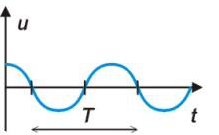
\includegraphics[width=0.5\textwidth]{Asin}
  \caption{Fala dźwiękowa.}
  \label{fig_dzwiek}
\end{figure}


Opisując nasze subiektywny odczucie dźwięku opisujemy go parametrami takimi jak : wysokość(zależy od częstotliwości), głośność(zależy od natężenia), barwa(zależy od widma fali akustycznej). Dźwięk w najprostszym przypadku może być pojedynczą sinusoidą(ton) o ustalonych parametrach amplitudy i częstotliwości, jednak w naturze mamy do czynienia z reguły w dźwiękami złożonymi(wielotonami). Wielotonem nazywamy sygnał będącym złożeniem sygnałów sinusoidalnych, mogą być one harmoniczne, którego składowe są krotnościami tonu podstawowego oraz nieharmoniczne gdzie taka zależność nie zachodzi, sygnały te są niezależne - w ludzkiej percepcji postrzegany jako szum.

Analizę dźwięku możemy przeprowadzać w dziedzinie czasu, sygnale takim jaki bezpośrednio potrafimy zarejestrować np. mikrofonem. Po dyskretyzacji sygnału do postaci cyfrowej dysponujemy ciągiem reprezentującym w pewnym przybliżeniu przebieg, w najprostszym ujęciu - sinusoidy(pojedynczego tonu). Posiadając tą wiedzę możemy zastosować szereg metod pozwalających na określenie częstotliwości dźwięku. Znacznym utrudnieniem dla tych metod będzie istnienie harmonicznych które mogą być mylące.

Innym podejściem, równie bardzo naturalnym jest transformacja sygnału z dziedziny czasu do dziedziny częstotliwości. Dzięki tej transformacji mamy bezpośrednio informację o częstotliwościach bazowych przetwarzanego sygnału. Jednak minusem badania sygnału w dziedzinie częstotliwości jest jego wrażliwość na szum, dlatego też dobrze poddać wstępnej filtracji z celu wyeliminowania szumu bądź przynajmniej jego zminimalizowaniu.


\subsection{Metoda w dziedzinie czasu : AMDF}


Metoda ta bazuje na porównaniu sygnału oryginalnego z opóźnionym. 
\begin{equation}
d(m) = \sum \limits ^{N-1} _{m=0} \| x(n) - x(n+m) \|
\end{equation}

Położenie pierwszego minimum funkcji $d(m)$ dla $m \neq 0$ wyznacza długość okresu najniższej składowej częstotliwościowej sygnału.

W najprostszym przypadku analizy pojedynczego tonu, metoda ta będzie sprawdzać się bezbłędnie, ponieważ porównując sygnał przesunięty z oryginalnym w momencie gdy wartość będzie równa 0 lub jej bardzo bliska, oznaczać to będzie jednakowość tych sygnałów lub znaczny stopień podobieństwa. Dlatego pierwsze minimum oznaczać będzie okres sinusoidy podstawowej sygnału. Pierwszym problemem może być szum, którego występowanie skutkować będzie spłyceniem minimów funkcji $d(m)$, jednak nadal będą one jednoznacznie określały okres częstotliwości dźwięku. W przypadku wielotonu spodziewać się możemy niejednoznaczności minimów, ponieważ składowe harmoniczne mogą się ,,znosić'', lokalnie powodując minima - fałszywe, funkcji d(m).

\subsection{Metoda w dziedzinie częstotliwości : analiza cepstralna}

Analiza cepstralna opiera się na obliczeniu cepstrum sygnału wejściowego. Czyli widma amplitudowego, widma amplitudowego sygnału wejściowego.

\begin{equation}
C(x) =\| FFT \left( ln \left( \| FFT(x) \| \right) \right) \|
\end{equation}


\begin{figure}[H]
  \centering
  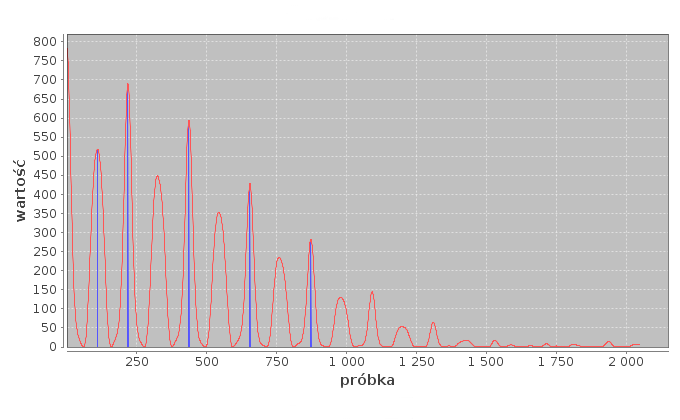
\includegraphics[width=0.7\textwidth]{cepstrum}
  \caption{Przykładowy wykres cepstrum.}
  \label{fig_cepstrum}
\end{figure}

Jak wspomniano na wstępie metoda ta jest wrażliwa na szum, wynika to z charakteru wykonywanej transformacji. Również jak w przypadku analizy dźwięku w dziedzinie czasu, składowe harmoniczne wielotonu będą powodować problemy w rozpoznawaniu częstotliwości podstawowej dźwięku. Jak widać na powyższym rysunku. Obok maksimów będących kolejnymi wielokrotnościami częstotliwości bazowej(maksymalny skok) występują pośrednie skoki, które w newralgicznych przypadkach mogą mieć wartość wyższą od skoku odpowiadającego częstotliwości bazowej, dlatego też zadanie to również nie zawsze da prawidłowy wynik. 


\section{Opis implementacji}


\subsection{Metoda w dziedzinie czasu : AMDF}

\subsection{Metoda w dziedzinie częstotliwości : analiza cepstralna}

Na podstawie analizy sygnałów wejściowych jak i odpowiadających im cepstrum, w drodze uzyskania jak najlepiej sprawdzającej się metody - ostatecznie otrzymaliśmy taki oto algorytm :

\begin{enumerate}
\item uśrednienie sygnału w celu zniwelowania wpływu szumu
\item ustawienie rozmiaru okna Hamminga na 4096
\item obliczenie transformaty fouriera aktualnie przetwarzanego fragmentu sygnału dyskretnego i wybranie widma mocy
$X = \| FFT(X) \|$
\item obliczenie logarytmu naturalnego kwadratu widma mocy sygnału
$X = log(\|X\| *\|X\|)$
\item obliczenie transformaty fouriera połowy otrzymanego sygnału(widmo jest symetryczne wystarczy jego połowa) i wybranie widma mocy
$C(X) = \| FFT(X) \|$
\item obliczenie kwadratu mocy widma
$X=C(X)*C(X)$
\item wybranie skoków najwyższych tak otrzymanego sygnału, nie tylko co do wartości, ale również najwyższych pod względem wysokości zbocza
\item wyznaczenie okresu dźwięku podstawowego na podstawie odległości pomiędzy dwoma kolejnymi najwyższymi skokami
\end{enumerate}

Ostatnie kroki są poprawką na podstawową wersję algorytmu niwelującą pewne niepożądane przypadku, tzn niezgodność maksymalnego lokalizacji maksymalnego skoku z oczekiwaną lokalizacją częstotliwości bazowej.


\section{Wyniki}


\subsection{Metoda w dziedzinie czasu : AMDF}

\subsection{Metoda w dziedzinie częstotliwości : analiza cepstralna}


\begin{table}[H]
\centering
\begin{tabular}{|c|c|c|c|}
\hline 
 \parbox{3cm}{lokalizacja\\ przewidywana} & \parbox{3cm}{lokalizacja\\ wyznaczona} & \parbox{3cm}{częstotliwość\\  przewidywana[Hz]} &  \parbox{3cm}{częstotliwość\\  wyznaczona[Hz]} \\
\hline
96 & 97 	& 455,00 & 454,64\\
\hline
43 & 43 	& 1025,00 & 1025,58\\
\hline
64 & 64 & 683,00 & 689,06\\
\hline
28 & 29 	& 1537,00 & 1520,69\\
\hline
490 & 490 & 90,00 & 90,00\\
\hline 
38 & 38 & 1139,00 & 1160,53\\
\hline 
196 & 196 & 225,00 & 225,00\\
\hline 
130 & 131 & 337,00 & 336,64\\
\hline 
551 & 276 & 80,00 & 159,78\\
\hline 
48 & 97 & 911,00 & 454,64\\
\hline 
119 & 120 & 369,00 & 367,50\\
\hline 
24 & 25 & 1779,00 & 1764,00\\
\hline 
159 & 81 & 276,00 & 544,44\\
\hline
49 & 49 & 887,00 & 900,00\\
\hline

\end{tabular} 
\caption{Wyznaczanie częstotliwości podstawowej w wybranych dźwiękach przykładowych.}
\label{wyniki:cepstrum}
\end{table}


\begin{figure}[H]
  \centering
  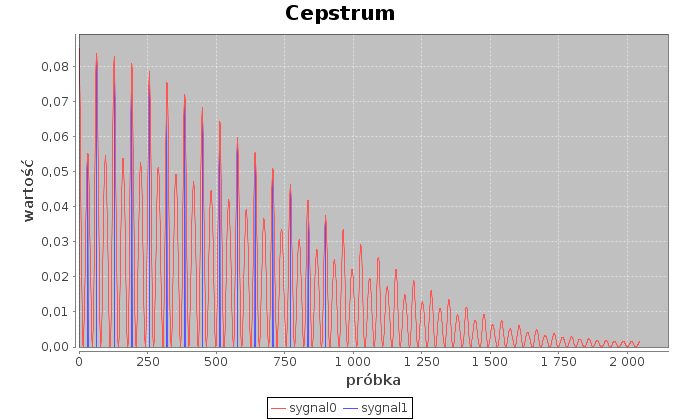
\includegraphics[width=0.7\textwidth]{cepstrum_viola_698}
  \caption{Wykres cepstrum dźwięku o częstotliwości 698Hz.}
  \label{fig_cepstrum698}
\end{figure}



\begin{figure}[H]
  \centering
  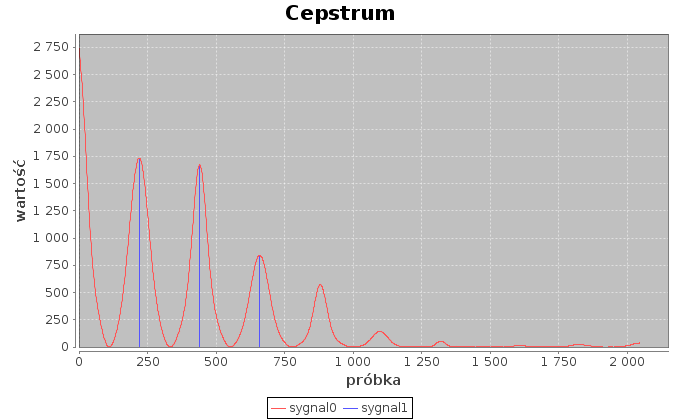
\includegraphics[width=0.7\textwidth]{cepstrum_artificial_100}
  \caption{Wykres cepstrum dźwięku o częstotliwości 100Hz.}
  \label{fig_cepstrum100}
\end{figure}


\section{Dyskusja}

\subsection{Metoda w dziedzinie czasu : AMDF}

\subsection{Metoda w dziedzinie częstotliwości : analiza cepstralna}

Jak widać w tabeli \ref{wyniki:cepstrum} metoda oparte o analize cepstralną radzi sobie dobrze z dźwiękami przykładowymi, również zadowalający - subiektywny, wynik otrzymaliśmy analizując sekwencje gry na wiolonczeli, gorzej poradziła sobie niestety z odtwarzaniem sekwencji gry na pianinie. Zauważalny problem który czasami występuje, jest identyfikacja jako częstotliwości podstawowych, wyższych lub niższych harmonicznych. Problem ten jest widoczny na rysunku \ref{fig_cepstrum100}. Pierwszy skok - maksymalny, w punkcie 220 wypada w połowie prawidłowej lokalizacji czyli 441. W zebranych danych w tabeli widoczny jest przypadek odwrotny czyli zidentyfikowanie częstotliwości dwa razy niższej od oczekiwanej.



\section{Wnioski}

Obie metody radzą sobie dobrze z powierzonym im zadaniem. Występują jednak przypadku które należałoby dokładniej przeanalizować w celu poprawy wyników odnajdywania częstotliwości podstawowej dźwięku. Napotkane problemy które mają wpływ na wyniki metod to złożoność dźwięku z wielu harmonicznych oraz szum który wydaje być się zjawiskiem naturalnym i nieodłącznym dla realnych przypadków.

Metoda oparta o analizę w dziedzinie częstotliwości wydaje się być dokładniejszą i mniej podatną na charakterystykę przetwarzanego dźwięku, czyli rodzaj i natężenie szumu i złożoność dźwięku.

Analiza cepstralna mimo, że z założenia powinna dawać wyniki łatwiejsze do interpretacji, to ze względu na zróżnicowanie sygnałów wejściowych nie jest jednak to zadaniem trywialnym. Zauważone i opisane problemy w sekcji dyskusji wskazują na problematyczność w interpretacji cepstrum. Również to, co nie było ujęte w dyskusji, zależność wyników tej metody od wielkości okna analizy. Pomijając przypadki oczywiste gdzie okno jest za małe z stosunku do okresu badanego dźwięku, przekształcenie sygnału do postaci cepstrum daje różne wyniki z zależności od wielkości okna.


\begin{thebibliography}{8}

\bibitem{1} Fast Fourier Transform (FFT) \url{http://www.cmlab.csie.ntu.edu.tw/cml/dsp/training/coding/transform/fft.html}
\bibitem{2} The Radix 2 Decimation In Frequency (DIF) Algorithm.  \url{http://www.engineeringproductivitytools.com/stuff/T0001/PT03.HTM}
\bibitem{3} !!!JAK COŚ ZNAJDZIESZ TO DODAJ!!! :P


\end{thebibliography}

\end{document}
